
\documentclass[letterpaper,hide notes,xcolor={table,svgnames},10pt]{beamer}
\def\showexamples{t}


%\usepackage[svgnames]{xcolor}

%% Demo talk
%\documentclass[letterpaper,notes=show]{beamer}

\usecolortheme{crane}
\setbeamertemplate{navigation symbols}{}

\usetheme{MyPittsburgh}
%\usetheme{Frankfurt}

%\usepackage{tipa}

\usepackage{hyperref}
\usepackage{graphicx,xspace}
\usepackage[normalem]{ulem}
\usepackage{multicol}
\usepackage{amsmath,amssymb,amsthm,graphicx,xspace}
\newcommand\SF[1]{$\bigstar$\footnote{SF: #1}}

\usepackage[default]{sourcesanspro}
\usepackage[T1]{fontenc}
\usepackage[scaled]{beramono}
\usepackage{tikzpagenodes}

\newcounter{tmpnumSlide}
\newcounter{tmpnumNote}


% old question code
%\newcommand\question[1]{{$\bigstar$ \small \onlySlide{2}{#1}}}
% \newcommand\nquestion[1]{\ifdefined \presentationonly \textcircled{?} \fi \note{\par{\Large \textbf{?}} #1}}
% \newcommand\nanswer[1]{\note{\par{\Large \textbf{A}} #1}}


 \newcommand\mnote[1]{%
   \addtocounter{tmpnumSlide}{1}
   \ifdefined\showcues {~\tiny\fbox{\arabic{tmpnumSlide}}}\fi
   \note{\setlength{\parskip}{1ex}\addtocounter{tmpnumNote}{1}\textbf{\Large \arabic{tmpnumNote}:} {#1\par}}}

\newcommand\mmnote[1]{\note{\setlength{\parskip}{1ex}#1\par}}

%\newcommand\mnote[2][]{\ifdefined\handoutwithnotes {~\tiny\fbox{#1}}\fi
% \note{\setlength{\parskip}{1ex}\textbf{\Large #1:} #2\par}}

%\newcommand\mnote[2][]{{\tiny\fbox{#1}} \note{\setlength{\parskip}{1ex}\textbf{\Large #1:} #2\par}}

\newcommand\mquestion[2]{{~\color{red}\fbox{?}}\note{\setlength{\parskip}{1ex}\par{\Large \textbf{?}} #1} \note{\setlength{\parskip}{1ex}\par{\Large \textbf{A}} #2\par}\ifdefined \presentationonly \pause \fi}

\newcommand\blackboard[1]{%
\ifdefined \showblackboard
  {#1}
  \else {\begin{center} \fbox{\colorbox{blue!30}{%
         \begin{minipage}{.95\linewidth}%
           \hspace{\stretch{1}} Some space intentionally left blank; done at the blackboard.%
         \end{minipage}}}\end{center}}%
         \fi%
}

\newcommand{\Rplus}{\protect\hspace{-.1em}\protect\raisebox{.35ex}{\small{\small\textbf{+}}}}
\newcommand{\CPP}{\mbox{C\Rplus\Rplus}\xspace}

%\newcommand\q{\tikz \node[thick,color=black,shape=circle]{?};}
%\newcommand\q{\ifdefined \presentationonly \textcircled{?} \fi}

\usepackage{listings,listings-rust}
\lstset{basicstyle=\footnotesize\ttfamily,
	breaklines=true,
	aboveskip=15pt,
  	belowskip=15pt,
	frame=lines,
	numbers=left, basicstyle=\scriptsize, numberstyle=\tiny, stepnumber=0, numbersep=2pt
}

\usepackage{siunitx}
\newcommand\sius[1]{\num[group-separator = {,}]{#1}\si{\micro\second}}
\newcommand\sims[1]{\num[group-separator = {,}]{#1}\si{\milli\second}}
\newcommand\sins[1]{\num[group-separator = {,}]{#1}\si{\nano\second}}
\sisetup{group-separator = {,}, group-digits = true}

%% -------------------- tikz --------------------
\usepackage{tikz}
\usetikzlibrary{positioning}
\usetikzlibrary{arrows,backgrounds,automata,decorations.shapes,decorations.pathmorphing,decorations.markings,decorations.text,decorations.pathreplacing}

\tikzstyle{place}=[circle,draw=blue!50,fill=blue!20,thick, inner sep=0pt,minimum size=6mm]
\tikzstyle{transition}=[rectangle,draw=black!50,fill=black!20,thick, inner sep=0pt,minimum size=4mm]

\tikzstyle{block}=[rectangle,draw=black, thick, inner sep=5pt]
\tikzstyle{bullet}=[circle,draw=black, fill=black, thin, inner sep=2pt]

\tikzstyle{pre}=[<-,shorten <=1pt,>=stealth',semithick]
\tikzstyle{post}=[->,shorten >=1pt,>=stealth',semithick]
\tikzstyle{bi}=[<->,shorten >=1pt,shorten <=1pt, >=stealth',semithick]

\tikzstyle{mut}=[-,>=stealth',semithick]

\tikzstyle{treereset}=[dashed,->, shorten >=1pt,>=stealth',thin]

\usepackage{ifmtarg}
\usepackage{xifthen}
\makeatletter
% new counter to now which frame it is within the sequence
\newcounter{multiframecounter}
% initialize buffer for previously used frame title
\gdef\lastframetitle{\textit{undefined}}
% new environment for a multi-frame
\newenvironment{multiframe}[1][]{%
\ifthenelse{\isempty{#1}}{%
% if no frame title was set via optional parameter,
% only increase sequence counter by 1
\addtocounter{multiframecounter}{1}%
}{%
% new frame title has been provided, thus
% reset sequence counter to 1 and buffer frame title for later use
\setcounter{multiframecounter}{1}%
\gdef\lastframetitle{#1}%
}%
% start conventional frame environment and
% automatically set frame title followed by sequence counter
\begin{frame}%
\frametitle{\lastframetitle~{\normalfont(\arabic{multiframecounter})}}%
}{%
\end{frame}%
}
\makeatother

\makeatletter
\newdimen\tu@tmpa%
\newdimen\ydiffl%
\newdimen\xdiffl%
\newcommand\ydiff[2]{%
    \coordinate (tmpnamea) at (#1);%
    \coordinate (tmpnameb) at (#2);%
    \pgfextracty{\tu@tmpa}{\pgfpointanchor{tmpnamea}{center}}%
    \pgfextracty{\ydiffl}{\pgfpointanchor{tmpnameb}{center}}%
    \advance\ydiffl by -\tu@tmpa%
}
\newcommand\xdiff[2]{%
    \coordinate (tmpnamea) at (#1);%
    \coordinate (tmpnameb) at (#2);%
    \pgfextractx{\tu@tmpa}{\pgfpointanchor{tmpnamea}{center}}%
    \pgfextractx{\xdiffl}{\pgfpointanchor{tmpnameb}{center}}%
    \advance\xdiffl by -\tu@tmpa%
}
\makeatother
\newcommand{\copyrightbox}[3][r]{%
\begin{tikzpicture}%
\node[inner sep=0pt,minimum size=2em](ciimage){#2};
\usefont{OT1}{phv}{n}{n}\fontsize{4}{4}\selectfont
\ydiff{ciimage.south}{ciimage.north}
\xdiff{ciimage.west}{ciimage.east}
\ifthenelse{\equal{#1}{r}}{%
\node[inner sep=0pt,right=1ex of ciimage.south east,anchor=north west,rotate=90]%
{\raggedleft\color{black!50}\parbox{\the\ydiffl}{\raggedright{}#3}};%
}{%
\ifthenelse{\equal{#1}{l}}{%
\node[inner sep=0pt,right=1ex of ciimage.south west,anchor=south west,rotate=90]%
{\raggedleft\color{black!50}\parbox{\the\ydiffl}{\raggedright{}#3}};%
}{%
\node[inner sep=0pt,below=1ex of ciimage.south west,anchor=north west]%
{\raggedleft\color{black!50}\parbox{\the\xdiffl}{\raggedright{}#3}};%
}
}
\end{tikzpicture}
}


%% --------------------

%\usepackage[excludeor]{everyhook}
%\PushPreHook{par}{\setbox0=\lastbox\llap{MUH}}\box0}

%\vspace*{\stretch{1}

%\setbox0=\lastbox \llap{\textbullet\enskip}\box0}

\setlength{\parskip}{\fill}

\newcommand\noskips{\setlength{\parskip}{1ex}}
\newcommand\doskips{\setlength{\parskip}{\fill}}

\newcommand\xx{\par\vspace*{\stretch{1}}\par}
\newcommand\xxs{\par\vspace*{2ex}\par}
\newcommand\tuple[1]{\langle #1 \rangle}
\newcommand\code[1]{{\sf \footnotesize #1}}
\newcommand\ex[1]{\uline{Example:} \ifdefined \presentationonly \pause \fi
  \ifdefined\showexamples#1\xspace\else{\uline{\hspace*{2cm}}}\fi}

\newcommand\ceil[1]{\lceil #1 \rceil}


\AtBeginSection[]
{
   \begin{frame}
       \frametitle{Outline}
       \tableofcontents[currentsection]
   \end{frame}
}



\pgfdeclarelayer{edgelayer}
\pgfdeclarelayer{nodelayer}
\pgfsetlayers{edgelayer,nodelayer,main}

\tikzstyle{none}=[inner sep=0pt]
\tikzstyle{rn}=[circle,fill=Red,draw=Black,line width=0.8 pt]
\tikzstyle{gn}=[circle,fill=Lime,draw=Black,line width=0.8 pt]
\tikzstyle{yn}=[circle,fill=Yellow,draw=Black,line width=0.8 pt]
\tikzstyle{empty}=[circle,fill=White,draw=Black]
\tikzstyle{bw} = [rectangle, draw, fill=blue!20, 
    text width=4em, text centered, rounded corners, minimum height=2em]
    
    \newcommand{\CcNote}[1]{% longname
	This work is licensed under the \textit{Creative Commons #1 3.0 License}.%
}
\newcommand{\CcImageBy}[1]{%
	\includegraphics[scale=#1]{creative_commons/cc_by_30.pdf}%
}
\newcommand{\CcImageSa}[1]{%
	\includegraphics[scale=#1]{creative_commons/cc_sa_30.pdf}%
}
\newcommand{\CcImageNc}[1]{%
	\includegraphics[scale=#1]{creative_commons/cc_nc_30.pdf}%
}
\newcommand{\CcGroupBySa}[2]{% zoom, gap
	\CcImageBy{#1}\hspace*{#2}\CcImageNc{#1}\hspace*{#2}\CcImageSa{#1}%
}
\newcommand{\CcLongnameByNcSa}{Attribution-NonCommercial-ShareAlike}

\newenvironment{changemargin}[1]{% 
  \begin{list}{}{% 
    \setlength{\topsep}{0pt}% 
    \setlength{\leftmargin}{#1}% 
    \setlength{\rightmargin}{1em}
    \setlength{\listparindent}{\parindent}% 
    \setlength{\itemindent}{\parindent}% 
    \setlength{\parsep}{\parskip}% 
  }% 
  \item[]}{\end{list}} 




\title{Lecture 29 --- Frontend Performance}

\author{Jeff Zarnett \\ \small \texttt{jzarnett@uwaterloo.ca}}
\institute{Department of Electrical and Computer Engineering \\
  University of Waterloo}
\date{\today}


\begin{document}

\begin{frame}
  \titlepage
 \end{frame}


\begin{frame}
\frametitle{Feelings and Facts}

Most topics of the course focus on how to actually improve the execution speed of the work to be done.

Frontend performance is unlike those kinds of improvements, because the user's feelings matter.

If they \textit{perceive} the page as fast, that's as good as, or better than, the page actually being faster.


\end{frame}


\begin{frame}
\frametitle{What Helps Perception}

\begin{enumerate}
	\item Acknowledgement of actions
	\item Loading spinners or progress bars
	\item Make the user \textit{think} it's done, even when it's not.
\end{enumerate}

\begin{center}
	
\includegraphics[width=0.7\textwidth]{images/isthatlegal.jpg}
\end{center}

\end{frame}


\begin{frame}
\frametitle{Thresholds}

Let's talk about the thresholds that matter to users: 
\begin{enumerate}
	\item Under 0.1 seconds is ``instant''.
	\item Between 1 and 10 seconds: use spinner	
	\item After 10 seconds, the user is impatient...
\end{enumerate}

Notify them? Send the result later?

\end{frame}


\begin{frame}
\frametitle{Motivation}

Aside from the correctness issues, there's also the risk that customers just... stop using your app or abandon whatever they were doing.

If it doesn't show up in voice of customer, is it a problem or do they just quit?

\end{frame}


\begin{frame}
\frametitle{Taking Too Long}

Study: users start abandoning the video load if it doesn't start in two seconds. 

Website speed: 4 s is perceived as long; 400 ms is correlated with lower usage.\\
\quad Tolerance depends on internet connection type.

Patience scales with what they asked for (e.g., GO Schedule vs Quest Report).

\end{frame}


\begin{frame}
\frametitle{Monetary Motivation}

\begin{center}
	
\includegraphics[width=0.4\textwidth]{images/getmoney.jpg}
\end{center}

Study: 0.1 second improvement in 15 retail brands' mobile website resulted in 8.4\% more conversions and 9.2\% higher order value.

\end{frame}


\begin{frame}
\frametitle{Is It Done?}

\begin{center}
	
\includegraphics[width=0.6\textwidth]{images/aurora.jpg}
\end{center}

\end{frame}


\begin{frame}
\frametitle{Trickery of Timing}

We'll also exclude from discussion things that look like only loading the first $n$ rows and then loading the rest when the user scrolls down.

What about showing the partial page as soon as we can?

Loading the shell helps a lot.

\end{frame}


\begin{frame}
\frametitle{Definitions}

\alert{FCP}: First Contentful Paint

\alert{LCP}: Largest Contentful Paint

These are measured in percentiles. You may look at 75th or 90th.


\end{frame}


\begin{frame}
\frametitle{First Contentful Paint}

\begin{center}
	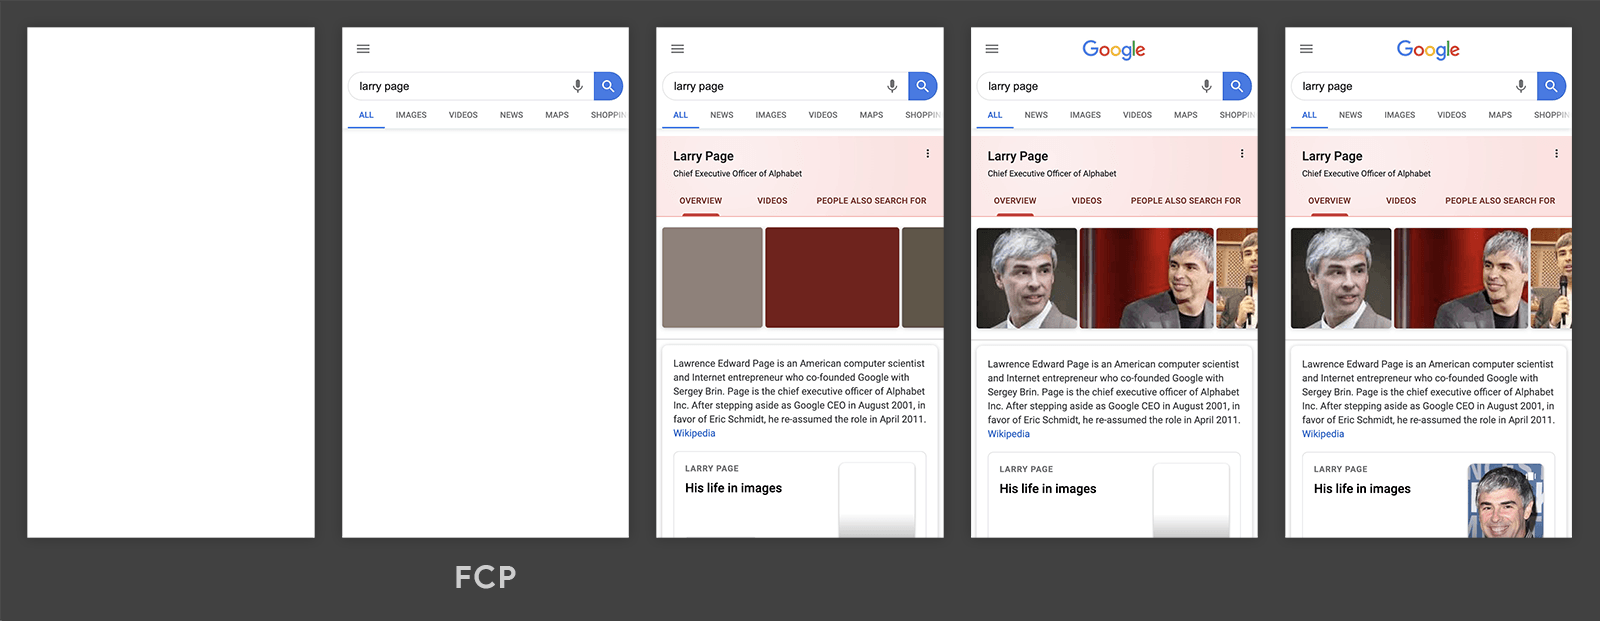
\includegraphics[width=\textwidth]{images/fcp.png}
\end{center}

\end{frame}


\begin{frame}
\frametitle{Largest Contentful Paint}

\begin{center}
	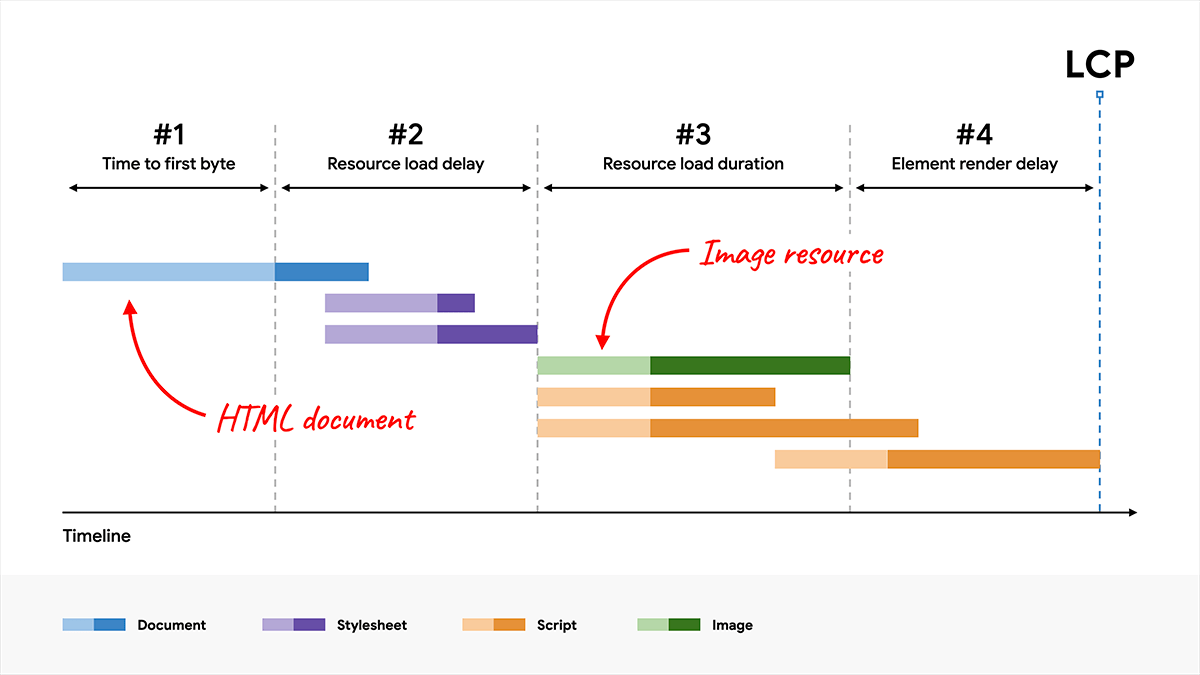
\includegraphics[width=\textwidth]{images/lcp-subparts.png}
\end{center}

\end{frame}


\begin{frame}
\frametitle{Which is the Largest?}

We might need to give the browser a hint what is the LCP.\\
\quad This is used by the preload scanner.

Preload scanner exists because the main parser can get blocked while working.\\
\quad Do things alongside this to look ahead and request what is needed.

Goal: prioritize the LCP element.


\end{frame}


\begin{frame}
\frametitle{Waterfall Loading}

\alert{Waterfall}: an unintentional sequence that should have been parallelized.

If we fetched data all at once we would save a lot of time.

Analogy: cooking without \textit{mise en place}.

\begin{center}
	
\includegraphics[width=0.3\textwidth]{images/distressed-gordon.jpg}
\end{center}

\end{frame}


\begin{frame}
\frametitle{Waterfall Loading}

It's the sequential nature of requests that's the problem, not the number of them.

Rather like the $N+1$ problem discussed much earlier, it is unlikely anyone sets out with the intention to write a waterfall.

It happens when there are nested components that depend on their parents.

\end{frame}


\begin{frame}
\frametitle{Do We Need It?}

If the parent element \textit{data} is needed, push this load into the backend.

If it's just the parent element \textit{render}, then use the \textit{mise en place} strategy: read the data tree first to find what to ask for.

\end{frame}


\begin{frame}
\frametitle{Rendering Pipeline}
Once the data is loaded, the next part we need to be concerned about is how to actually render this efficiently. 

If we assume that the user's display refreshes 60 times per second, a frame render needs to take place in about 10~ms, otherwise the page stutters.

This is sometimes referred to as ``jank''.

\end{frame}


\begin{frame}
\frametitle{Steps}

Browser is mostly sequential, with limited parallelism.

\begin{enumerate}
	\item JavaScript
	\item Style
	\item Layout
	\item Paint
	\item Composite
\end{enumerate}

Goal: make the changes so that the browser starts at the latest stage possible.

\end{frame}


\begin{frame}
\frametitle{Shimmer}

Consider a text shimmer example!

If the code changes background-position, this forces a repaint on every frame, so it requires more CPU time. 

Animate a transform: the text is painted one time and the work is just composition: slide the overlay over a bit and stack the elements again. 

That's not for free, though, because the overlay needs to have its own layer, which takes up more memory.

\end{frame}


\begin{frame}
\frametitle{Cumulative Layout Shift}

Sounds the same, but actually different: \alert{cumulative layout shift}. 

Perhaps you've had the experience on a webpage where you go to click on something and the page moves and you end up clicking the wrong thing? 

This is a bad user experience, but it's not the focus of this section.

\end{frame}


\begin{frame}
\frametitle{Reduce Work}

If big changes are not necessary, don't do them.

We can think of the previous frame not only as the initial state, but also as cached results.

Minor changes invalidate a small part of it; major changes force more work.

\end{frame}


\begin{frame}
\frametitle{Layout Thrashing}

\alert{Layout thrashing} is the term for many forced layouts in quick succession. 

The most efficient way for the browser to do the work it needs is to wait for all the changes to take place, then do the layout once. 

If we don't do that, we end up repeating a lot of work unnecessarily.


\end{frame}


\begin{frame}[fragile]
\frametitle{Layout Thrashing}

\begin{lstlisting}
function resizeAllParagraphsToMatchBlockWidth () {
  // Puts the browser into a read-write-read-write cycle.
  for (let i = 0; i < paragraphs.length; i++) {
    paragraphs[i].style.width = `${box.offsetWidth}px`;
  }
}
\end{lstlisting}



\begin{lstlisting}
// Read.
const width = box.offsetWidth;

function resizeAllParagraphsToMatchBlockWidth () {
  for (let i = 0; i < paragraphs.length; i++) {
    // Now write.
    paragraphs[i].style.width = `${width}px`;
  }
}
\end{lstlisting}

\end{frame}


\begin{frame}
\frametitle{Modelling}
All of this describes the work required to render one frame! 


A webpage has a \alert{Document Object Model (DOM)} that represents the structure.

Google's Lighthouse performance tool considers the DOM to be a warning-level of complex at 800 nodes and an error-level of complex at 1400.

\end{frame}


\begin{frame}
\frametitle{Simplify the DOM}

Simplifying the DOM is an obvious strategy: if there's less loaded on the page, there's less to do. 

This may also result in less data being required from the backend, which then improves the data loading time. Two for one. 

But if you need all the data on the page, it's hard to cut this down.

\end{frame}


\begin{frame}
\frametitle{Virtualization}

If we can't reduce the data, the plan is \alert{virtualization}.

It means only creating elements for things that are visible on screen. 
 
Imagine a calendar with hundreds of appointments; they can't all fit on screen.
 
 The tradeoff, though, is that elements that are virtualized are not in the DOM so we can't find them with a search. 

\end{frame}

\begin{frame}
\frametitle{Virtualization}

Render them later?

There exists the \texttt{content-visibility} property in CSS that lets things be rendered on demand.

It reduces the work done on an initial page render and skips re-rendering for things that aren't visible.

\end{frame}



\begin{frame}
\frametitle{How Much to Redraw?}

If one data element is updated: risk that it forces a very large re-load/re-render. 


Calendar example: change 1 appointment from 9:00 to 9:30. 

If subscribed to the collection, the whole collection ``changed''.\\
\quad General tree comparison is $O(n^{3})$ but even $O(n)$ is bad.


\end{frame}


\begin{frame}
\frametitle{False Sharing}
Subscribing to the entire collection results in something that resembles false-sharing!

Appointments are in a lookup table by ID and there's a separate list of IDs?

The calendar component needs to look at the list of IDs and create one component per ID; that component gets its data from the table.

\end{frame}



\begin{frame}
\frametitle{What Makes for Good IDs?}

If the data element itself has a unique ID (e.g., account number), good choice.

If we go by position in the list, it makes re-ordering a pain. 

Random or unstable IDs are the worst choice because we could end up with a lot of unnecessary re-creation of elements.

\end{frame}


\begin{frame}
\frametitle{Not So Different}

Get LCP done earlier and then call that ``done'' is a little bit unusual.

Everything else about frontend performance relates nicely to other things we've covered in the course!

Move things off the critical path, do less work, and trade space for time. 


\end{frame}



\end{document}
